\documentclass[a4paper,man]{apa6}

\usepackage[english]{babel}
\usepackage[utf8x]{inputenc}
\usepackage{amsmath}
\usepackage{graphicx}
\usepackage[colorinlistoftodos]{todonotes}
\usepackage{tikz}
\usepackage{tikz-qtree}
\usepackage{caption}
\usepackage{subcaption}
\usepackage{pslatex}
\usepackage{apacite}
\usepackage{float}

\newcommand{\key}[1]{\emph{#1}}
\newcommand{\denote}[1]{\mbox{ $[\![ #1 ]\!]$}}

\title{Incremental understanding of conjunctive generic sentences}
\shorttitle{elephants}
\author{Michael Henry Tessler, Karen Gu, and Roger Levy}
\affiliation{Department of Brain and Cognitive Sciences, MIT}

\abstract{Generic statements convey generalizations about categories, but how generic predications combine is unclear.
``Elephants live in Africa and Asia'' does not mean that individual elephants live on both continents.
In addition, such conjunctive generics pose interesting questions for theories of incremental processing because the meaning of the sentence can change part-way through: ``Elephants live in Africa'' would imply most or all do, but ``Africa and Asia'' implies some live in each. 
We extend a recently proposed computational model of generic language understanding with an incremental processing mechanism that can begin to interpret an utterance before a speaker has finished their sentence.
This model makes novel predictions about partial interpretations of conjunctive generic sentences, which we test in two behavioral experiments. 
The results support a strong view of incrementality, wherein listeners continuously update their beliefs based on expectations about where a speaker will go next with their utterance.

\textbf{Keywords:} 
semantics; pragmatics; incremental processing; generics; psycholinguistics}

\begin{document}

\maketitle


\section{Introduction}


Much of what we come to learn about the world comes not from direct experience but from knowledge conveyed to us from others, often in the form of linguistic utterances. 
``Elephants eat 300 pounds of a food in a day'' succinctly conveys information extending beyond any particular moment in time or space: It could apply to any elephant, on any day of the week. 
Utterances that communicate generalizations are called \emph{generic} utterances \cite{Carlson1977, genericBook}, and they are the foremost case study of rich, abstract knowledge conveyed in simple utterances \cite{Gelman2009}.

Generics are rife with philosophical puzzles that make it difficult to develop a unified, formal theory of their meaning \cite<for useful reviews:~>{genericBook, Nickel2016}.  One largely understudied puzzle concerns how generic predications combine.  Consider the null hypothesis that generics convey information about the percentage of the category with the property---the \key{prevalence}---in a way analogous to how majority quantifiers (e.g., \emph{most}, \emph{all}) work (e.g., ``Most elephants eat 300 pounds of food in day''). 
How can such an account treat a generic involving a conjunctive predication like ``Elephants live in Africa and Asia''?  No elephant actually lives on both continents; instead, the sentence should be understood as  \emph{(generically) elephants live in Africa and (generically) elephants live in Asia}, but this is impossible if each individual generic sentence means that the majority holds the property \cite<i.e., it is impossible for more than half of elephants to live in Africa and more than half of elephants to live in Asia;>{Nickel2008}. 
The prevalence implied by a generic involving a conjunctive, mutually-exclusive predicate seems more lax than if only one of conjuncts were mentioned: If a speaker said ``Elephants live in Africa'', you might think they all do. 

The puzzle of understanding conjunctive generic sentences deepens when one considers that linguistic input is processed incrementally \cite<e.g.,>{Altmann1999}: Listeners ubiquitously form expectations about the intended meaning of a sentence before the speaker finishes it \cite<e.g.,>{tanenhaus1995integration}.  For conjunctive generics about mutually exclusive properties, strongly incremental language understanding might produce non-monotonic belief updates: after the sentence prefix ``Elephants live in Africa\ldots'', a comprehender might infer a higher prevalence than after hearing the sentence completion ``\ldots and Asia''.  If such non-monotonic updates occur, what types of linguistic input trigger them?  

In this paper we show that a recently proposed model of generic language can accommodate these complex inferential patterns and we empirically test two predictions about generic interpretation that address these puzzles.  The model of \citeA{Tessler2019:genLang} treats generics as a kind of vague quantifier: interpretation of a generic depends on prior beliefs about properties. First, we show how when properties are likely to be mutually incompatible (as in \emph{live in Africa and Asia}), listeners infer lower prevalences of each property following a conjunctive generic sentence than when the properties are compatible. Second, we show how the above model, when integrated with expectation-based probabilistic theories of syntactic processing \cite{hale:2001,Levy2008}, predicts that comprehenders update their beliefs about property prevalence not just when encountering a second, conjoined property, but immediately upon encountering evidence that a second, conjoined property is likely to be forthcoming.  We test these predictions in two behavioral experiments that probe listeners' understanding of conjunctive generic sentences at different points mid-sentence, analogous to gating paradigms in psycholinguistics \cite{Grosjean1980}.  Our empirical data confirm both predictions, suggesting that generic language interpretation interacts jointly with world knowledge and strongly incremental syntactic processing according to principles of probabilistic inference under uncertainty.

\begin{figure*}[t]
  \centering
    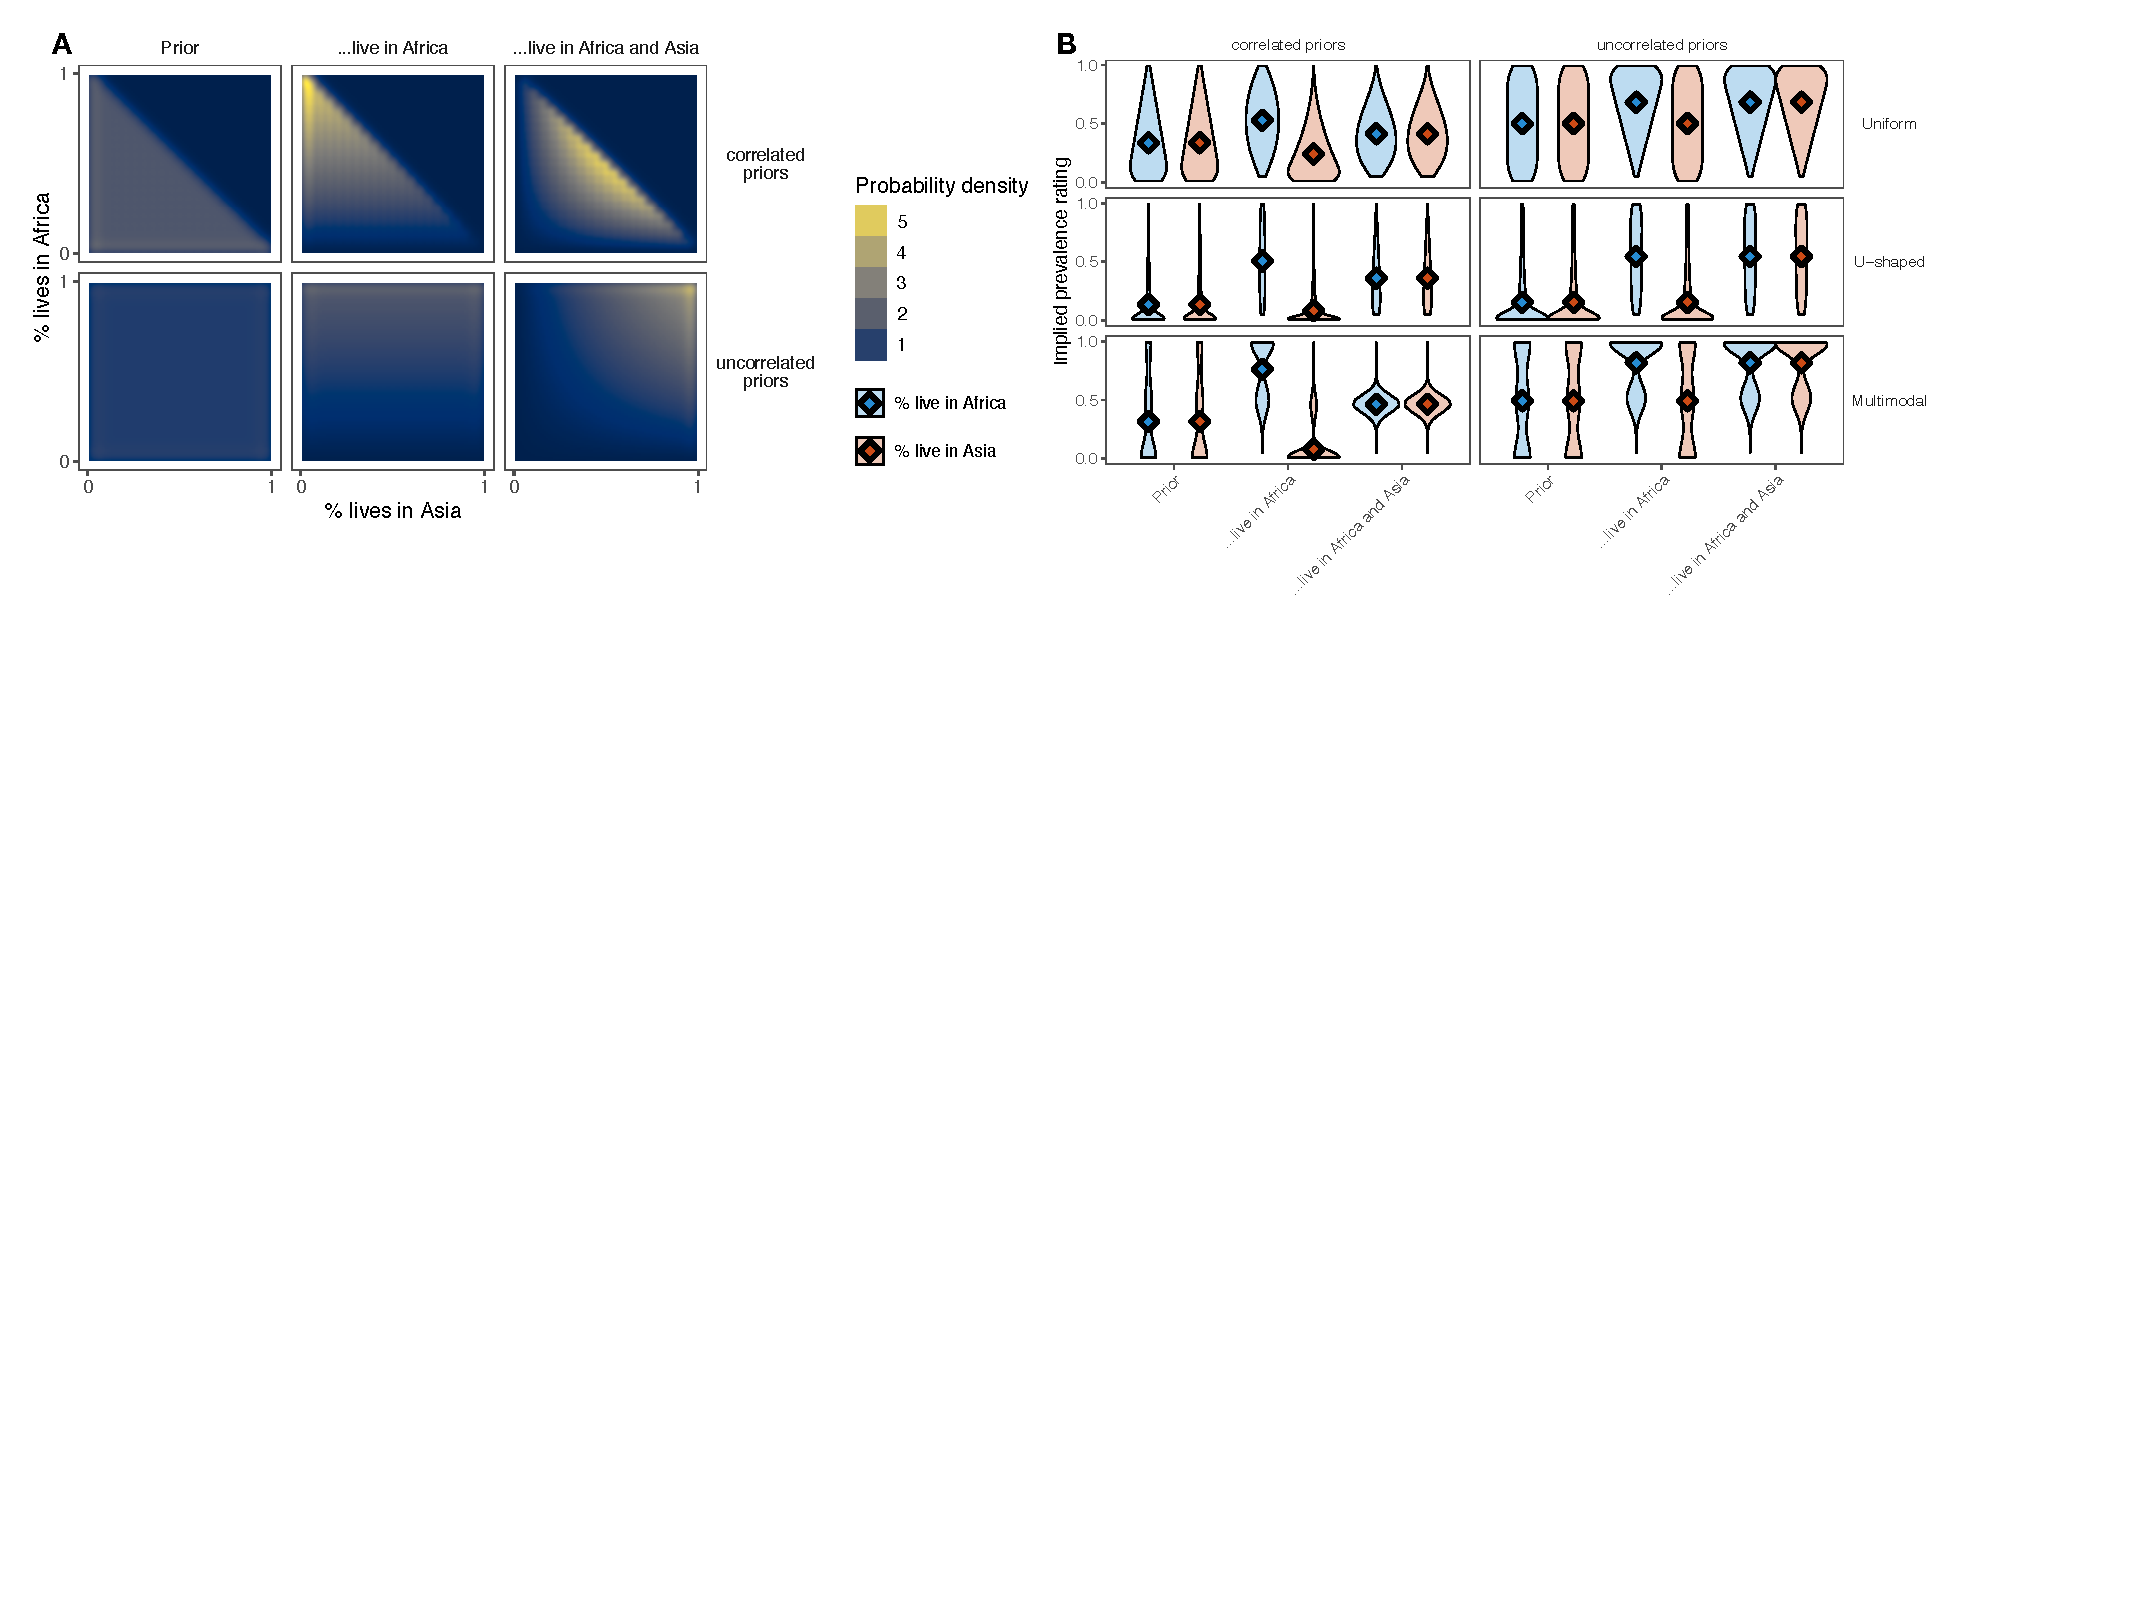
\includegraphics[width=1\textwidth]{figs/model.pdf}
  \caption{Model's sequential interpretation of ``Elephants live in Africa\ldots and Asia.'' A: Correlated priors reflected in the joint probability distribution over two features result in a mutual exclusivity inference. When the model hears only ``\ldots live in Africa'', it believes that probably all live in Africa (middle facet); when it hears they live in Asia as well, the model non-monotonically updates its beliefs about how many live in Africa. B: The mutual exclusivity inference holds for priors of different shapes and never holds if the prior knowledge about the two features is uncorrelated. Points show means of distributions. U-shaped priors were Beta(0.1, 1); multimodal priors were an equal mixture of a Beta(1, 100) and a Beta(25, 1). Correlated priors were created by adding an additional factor that decreased the probability of a prevalence-level if the sum of the prevalence of the two features exceeded 100\%. }
  \label{fig:model}
\end{figure*}


\section{Computational Model}


We extend a model for interpreting generics to incorporate an incremental processing mechanism that allows a listener to understand partial utterances.
The original model of \citeA{Tessler2019:genLang} interprets a generic utterance predicating a property of a category (``Elephants eat 300 pounds of food in a day'') as meaning that the prevalence (or probability) $x$ of the property given the category---$P($eats 300 lb. of food in a day$\mid$ is an elephant$)$---is greater than an \emph{a priori} uncertain threshold $\theta$.
The literal meaning of the generic---an uncertain threshold function, with uniform uncertainty over the threshold $P(\theta$)---combines with a listener's prior knowledge about the prevalence of the feature $P(x)$ within a relevant set of alternative categories (e.g., other animals) to compute a posterior distribution over prevalence $x$:

\begin{equation}
P(x \mid u) = \int_{\theta} P(x, \theta \mid u)  d\theta \propto P(x) \cdot P(\theta) \cdot \delta_{\denote{u}(x, \theta)} 
\label{eq:L0}
\end{equation}
\noindent where $\delta_{\denote{u}(x, \theta)}$ is the Kronecker delta function assigning a value of 1 for utterances that are literally true (in the case of a generic: where $x > \theta$) and 0 for utterances that are false.


To interpret a generic with a conjunctive predicate such as ``Elephants live in Africa and Asia'', we assume the semantic representation contains a conjunction of two generic statements:
$
[Gen(\textnormal{elephant})( \textnormal{live\_in\_Africa})] \land
[Gen(\textnormal{elephant})( \textnormal{live\_in\_Asia})],
$
where the $Gen$ operator acts according to the belief-updating rule of Eq.~\ref{eq:L0} (see \citeA{Nickel2008} for supporting arguments of this semantic parse).
A listener starts with a joint prior over the prevalence of the two properties (we denote variables associated with \emph{living in Africa} with subscript $r$ and \emph{Asia} with $s$): $P(\textbf{x}) = P(x_{r}, x_{s})$, which is incrementally updated with each successive generic. 
The model can then interpret multiple generics in succession, using the posterior distribution over prevalence $P(\textbf{x} \mid u)$ (Eq.~\ref{eq:L0}) as the prior for the next utterance. 
\begin{equation}
P(\textbf{x} \mid u_{r}, u_{s}) \propto  \int_{\theta_s} \int_{\theta_r}P(\textbf{x}, \boldsymbol{\theta} \mid u_{r})  \cdot \delta_{\denote{u_{s}}(x_{s}, \theta_{s})} d\theta_r d\theta_s%\\
\label{eq:L0a}
\end{equation}
\noindent where $P(\textbf{x}, \boldsymbol{\theta} \mid u_{r})$  is the posterior that results from hearing ``Elephants live in Africa'' given by Eq.~\ref{eq:L0}.

The predictions for a sequential understanding of ``Elephants live in Africa and Asia'' are shown in Fig.~\ref{fig:model}.
Upon hearing the first part of the utterance, the model believes that almost all elephants live in Africa (simulations assuming a uniform prior shown in Fig.~\ref{fig:model}A). 
What happens next depends upon the correlational structure of the prevalence prior: If the listener has prior knowledge suggesting the properties (living in Africa, living in Asia) are mutually exclusive (Fig.~\ref{fig:model}A top), they interpret the next part of the utterance (``...and Asia'') as indicating that some (perhaps half) of elephants live in Africa and other ones live in Asia. 
Without this correlation in the prior, the model ends up believing that most or all elephants live both in Africa and in Asia  (Fig.~\ref{fig:model}A bottom).
These inferences are robust to a variety of different prevalence prior distributions, so long as the prior has the necessary correlational structure (Fig.~\ref{fig:model}B shows predictions assuming a uniform, U-shape Beta, and mixture-of-Beta distributions).


\begin{figure}
  \definecolor{darkgreen}{RGB}{0,100,0}
    \definecolor{lightgreen}{RGB}{144,238,144}
\tikzset{sibling distance=-3pt, level distance=16pt}
  \centering
\scriptsize
\begin{tabular}{cc}
  \hspace{-0.25cm}
 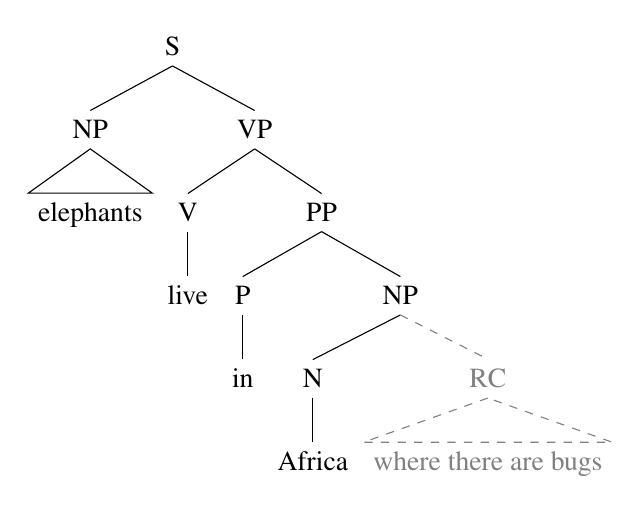
\begin{tikzpicture}
	        \Tree [.S [.NP \edge[roof]; elephants ]
	                  [.VP [.V live ] [.PP [.P in ] [.NP [.N Africa ] \edge[color=gray, style=dashed]; [.{\textcolor{gray}{RC}} \edge[color=gray, style=dashed, roof]; {\textcolor{gray}{where there are bugs}} ] ] ] ] ]
\end{tikzpicture}
&\hspace{-1.25cm}
 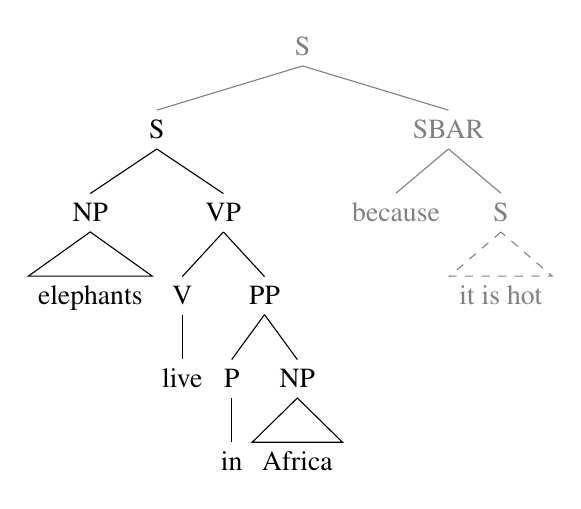
\begin{tikzpicture}[sibling distance=0pt]
	        \Tree [.{\textcolor{gray}{S}} \edge[color=gray]; [.S [.NP \edge[roof]; elephants ]
                [.VP [.V live ] [.PP [.P in ] [.NP \edge[roof]; Africa ] ] ] ]
                \edge[color=gray];
                [.{\textcolor{gray}{SBAR}} \edge[color=gray];  \textcolor{gray}{because} \edge[color=gray]; [.{\textcolor{gray}{S}} \edge[color=gray,style=dashed, roof]; {\textcolor{gray}{it is hot}} ] ] ]
\end{tikzpicture}
  \\
    \hspace{-0.5cm}
      \begin{tikzpicture}[sibling distance=0pt]
	        \Tree [.S [.NP \edge[roof]; elephants ]
	                  [.VP [.V live ] [.PP [.P in ]
	                       	[.NP [.NP Africa ] 
                                 \edge[color=darkgreen]; [.\textcolor{darkgreen}{Conj} \textcolor{darkgreen}{and} ]
		                       	\edge[color=lightgreen, style=dashed]; [.\textcolor{lightgreen}{NP}  \edge[color=lightgreen, style=dashed, roof]; \textcolor{lightgreen}{Asia} ]] ] ]]
\end{tikzpicture}
    & \hspace{-1cm}
\begin{tikzpicture}[sibling distance=0pt]
	        \Tree [.S [.NP \edge[roof]; elephants ]
	                  [.VP [.VP \edge[roof]; {live in Africa} ]
                               \edge[color=darkgreen]; [.\textcolor{darkgreen}{Conj} \edge[color=darkgreen]; \textcolor{darkgreen}{and} ] 
				\edge[color=lightgreen, style=dashed]; [.\textcolor{lightgreen}{VP}  \edge[color=lightgreen, style=dashed, roof]; \textcolor{lightgreen}{eat bugs}
				] ] ]
\end{tikzpicture}
\end{tabular}
\caption{Incremental parse trees and syntactic expectations for upcoming conjunct properties in generic predication.  The string prefix ``Elephants live in Africa\ldots'' is compatible with a variety of continuations, including the four listed above.  The next word, ``\textcolor{darkgreen}{and}'', rules out the continuations in the top row (depicted in gray) and sharpens expectations around a conjunct at potentially different structural levels (light green).  Probabilistic renormalization implies that an upcoming conjunct mutually exclusive with the first conjunct becomes more likely when ``and'' is encountered, driving the strong incremental predictions depicted in Fig.~\ref{fig:incremental}.}
\label{fig:trees}
\end{figure}


When processing a conjunctive phrase, listeners may form expectations about the complete utterance even before the sentence is over. 
For example, when a speaker reaches the word \emph{Africa} in ``Elephants live in \emph{Africa}'', she has many syntactically distinct options available to her to complete the sentence (Fig.~\ref{fig:trees} shows four possibilities).
One such possibility is that she continues with a NP-coordination that includes a mutually exclusive property (e.g., \emph{and Asia}; bottom-left tree). 
When the listener encounters the word \emph{and} in ``Elephants live in Africa \emph{and}'', he knows he is entering into a coordination and the relative probability of a forthcoming mutually exclusive property increases.
Such a continuation would yield a different inference about the prevalence of elephants in Africa than a continuation with a non-mutually exclusive property (e.g., with a verb phase such as ``and eat bugs'').\footnote{
	For illustrative purposes, we assume a correlation between NP~vs.~VP coordination and mutually exclusive~vs.~non-mutually exclusive predicates. Of course, it is possible to continue with a verb phrase about a mutually exclusive property such as ``\ldots live in Africa and live in Asia'' as well as continue with a noun phrase about a non-mutually exclusive property (e.g., ``\ldots eat figs and nuts''). The crucial fact is that the probability of a forthcoming mutually-exclusive property increases when the comprehender encounters the word \emph{and}. 
}
If listeners parse and interpret utterances incrementally at the level of individual words, then we would expect their inferences about the prevalence of elephants in Africa to represent a mixture of the inferences derived from different possible continuations, which can be represented by conditional probabilities of the full utterance $u'$ given the sentence fragment heard $f$:

\begin{equation}
P(x \mid f) = \sum_{u'} P(x \mid u') P(u' \mid f) 
\label{eq:L0a}
\end{equation}

If, however, listeners do not derive incremental interpretations at each moment, but instead wait for meaningful pieces of an utterance (e.g., content words like \emph{Asia}) to compute interpretations, then we would not expect such an intermediate degree of interpretation: ``Elephants live in Africa and\ldots'' should mean the same thing as ``Elephants live in Africa\ldots'' (Fig.~\ref{fig:incremental}). 
We test this prediction in Expt.~2 using a gating paradigm in the spirit of \citeA{Grosjean1980}.






\begin{figure}[t]
  \centering
    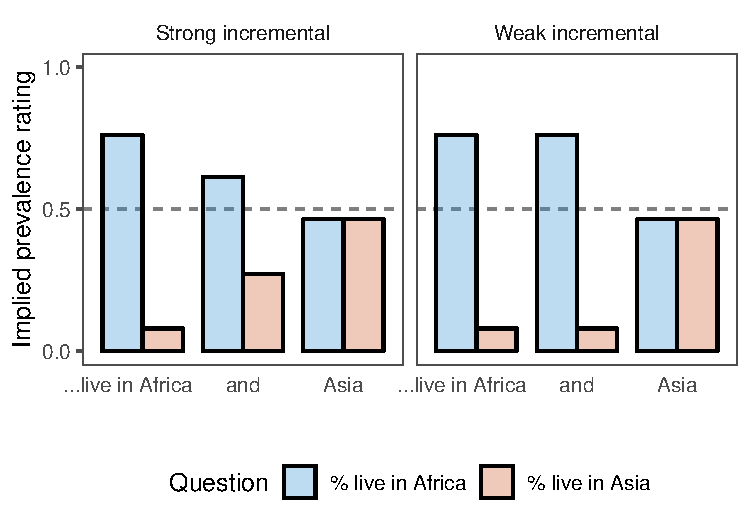
\includegraphics[width=0.5\textwidth]{figs/incremental.pdf}
    \vspace{-0.5cm}
  \caption{A model that incorporates syntactic expectations at the level of individual words (\emph{strong incremental}) predicts intermediate mutual-exclusivity inferences part-way through the conjunction (at ``and''), whereas a model that waits for content-words (\emph{weak incremental}) does not show a difference in expected prevalence at the word ``and.''
  }
          \vspace{-0.3cm}
  \label{fig:incremental}
\end{figure}


\section{Experiments}

We design two experiments to test the mutual exclusivity (ME) and incremental predictions.
Expt.~1 tests the ME prediction that ``Elephants live in Africa and Asia'' means roughly that half live in Africa and half live in Asia; this experiment also serves to validate the gating procedure we employ in the second experiment. 
Expt.~2 is a pre-registered study that uses the gating paradigm to test the fine-grained incremental predictions of the model.
The experiments and a full list of materials can be viewed at \url{tinyurl.com/elephants-cogsci}.


\begin{figure*}[h]
  \centering
    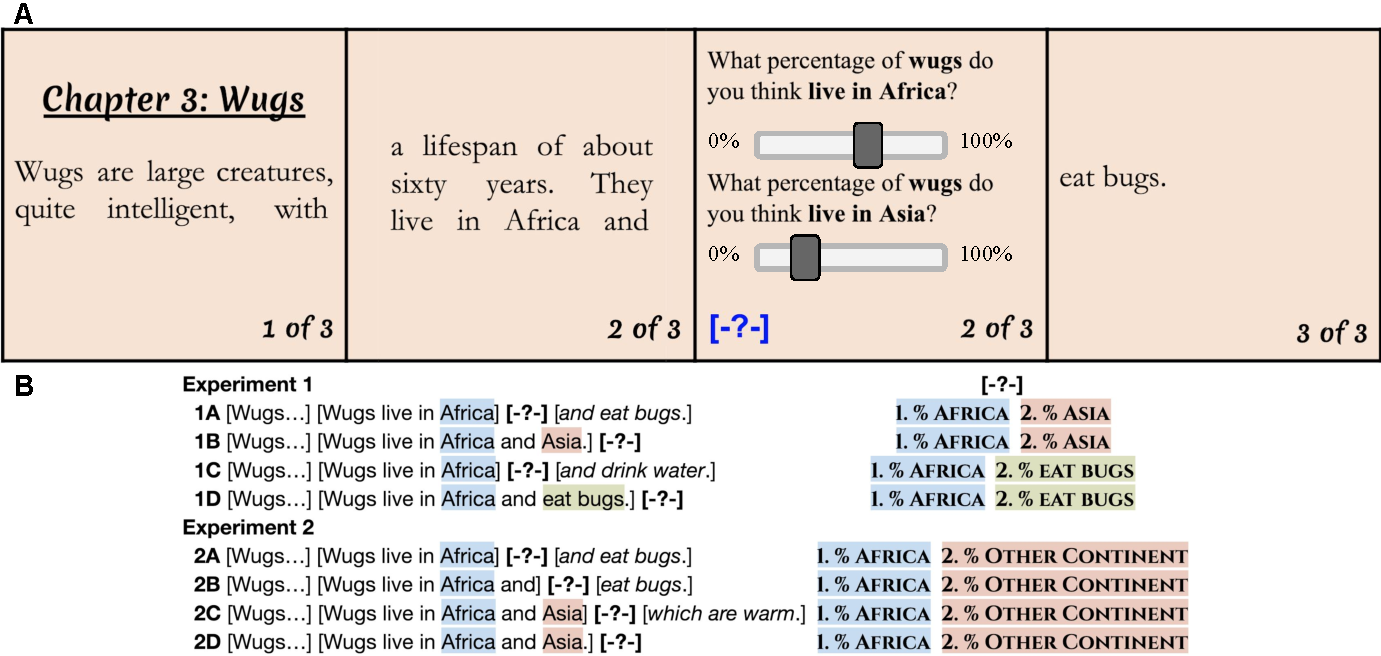
\includegraphics[width=1\textwidth]{figs/design.pdf}
    \vspace{-0.5cm}
  \caption{Overview of experiments. A: Example book chapter from Expt.~2, depicting the \emph{Interrupted A\&} condition. ``Africa and Asia'' property is shown for illustration; actual stimuli used novel names for properties (``Caro and Este''). B: Overview of conditions for Expts.~1 and 2. [-?-] denotes point in the sentence at which the question appeared. Highlighting shows which properties were mentioned before the question, and what was asked about. See main text for full description of conditions.}
  \label{fig:design}
          \vspace{-0.5cm}
\end{figure*}

\subsection{Experiment 1: Mutual exclusivity inference}

\subsubsection{Participants}

We recruited 27 participants through Amazon's Mechanical Turk.
Participants were restricted to those with verified U.S. IP addresses and at least a 95\% work approval rating. 
The study took about 10 minutes and participants were compensated \$1.50.

\subsubsection{Materials}

Participants read a storybook with chapters about creatures on a faraway planet.
Each chapter contained a short paragraph presented across 2--4 screens, with a button to ``turn the page'' (Fig.~\ref{fig:design}A).
A chapter introduced one or a few novel categories (e.g., \emph{wugs}) and semi-novel properties (e.g., \emph{live on the continent of Caro}).
Critical trial chapters ended with a generic sentence about conjunctive properties, which differed only in whether the second property was mutually exclusive with the first (\emph{conjunct type}): ``Glippets live on the continent of Caro and \emph{on the continent of Este} (ME) /  \emph{enjoy the sunshine there} (not ME: NME).''

The earlier content of the chapter supported the mutually exclusive interpretation of the properties when the properties were not \emph{ipso facto} mutually exclusive. For example: 

\begin{quote}
\small
Krens are a tribe of the aliens that live on the continent of Benli. Animals like stups, four-legged creatures with large antlers, are a resource for the Krens. Stups roam all over the windy highlands of Benli, far from the oceans. Krens are stup-herders and (\emph{fishermen} / \emph{incorporate stups into their religion}).
\end{quote}


\noindent Conjunct type (ME~vs.~NME) was manipulated within participants and items. 
There were 14 filler chapters with content similar to the critical chapters but using explicit quantifiers (\emph{most}, \emph{all}, \emph{none}) to describe the properties of categories.


\subsubsection{Procedure}
Participants were told they would be reading a storybook with a question in each chapter. 
Questions were all of the same type, an \emph{implied prevalence} question \cite{Gelman2002, Cimpian2010}: ``What percentage of Ks do you think F?'', where K represents a category and F a feature. 
Responses were recorded using a slider with endpoints labeled 0\% and 100\%, with the exact value selected appearing above the slider. 
Participants were familiarized with the response variable in a practice trial, where they were asked to report how many \emph{dogs bark}, \emph{birds are male}, \emph{cats get cancer}, and \emph{lions lay eggs}. 
These questions encouraged participants to use the full range of the response scale as well as served as a comprehension check. 

In each critical chapter of the storybook, two questions appeared either at the end of the chapter (\emph{Uninterrupted} conditions) or interrupting the chapter right before the final page  (\emph{Interrupted} conditions; Fig.~\ref{fig:design}).
In the Interrupted conditions, the question came in the middle of a conjunctive generic sentence, but before the conjunction so the reader was unaware the sentence would continue with a conjunction.
The questions asked about the mentioned property (e.g., \emph{Africa}) and either a mutually exclusive property (\emph{Asia}; \emph{ME} conditions) or a nonmutually exclusive property (e.g., \emph{eats bugs}; \emph{NME} conditions); the chapter then concluded with a conjunction about an unmentioned, nonmutually exclusive property (Fig.~\ref{fig:design}B), so as to not give the impression that the participant was being tricked by being asked about a property that we would eventually reveal.
In the critical trials,  the second question was asked about the second property mentioned (ME~vs.~NME). 
Filler trials asked about two properties described in the chapter using quantifiers (i.e., \emph{all}, \emph{most}, or \emph{none}).
The order in which the two questions appeared on the screen was randomized on each trial.

Each participant read a total of 21 chapters, which included 8 ME conjunctions, 4 NME conjunctions, and 6 quantifier fillers; for each of these categories, equal numbers of interrupted and uninterrupted were used. 
The experiment began with a chapter with no questions and 2 filler trials; the remaining trials were presented in a random order such that no two critical trials were presented back-to-back. 
Subjectively, the task is very difficult as participants learn about many different animals with lots of new names; in practice, however, participants only need to recall information from the previously encountered sentence to answer the trial questions. 
Following the storybook, participants completed a memory check where they had to select all the facts they had learned from a list of 10 (5 real, 5 distractor); in addition, participants were asked to explain what the experiment was about in broad terms.



\subsubsection{Results}




11 participants were excluded for failing to respond accurately to all of the practice trials or  failing to respond accurately to at least 7 of the 10 memory check prompts (same exclusion criteria for Expt.~2).
We describe the results using the running example of ``Elephants live in Africa and Asia'', but the experimental stimuli used novel categories and relatively novel properties.

 \vspace{-0.5cm}
 \begin{figure}[h]
  \centering
    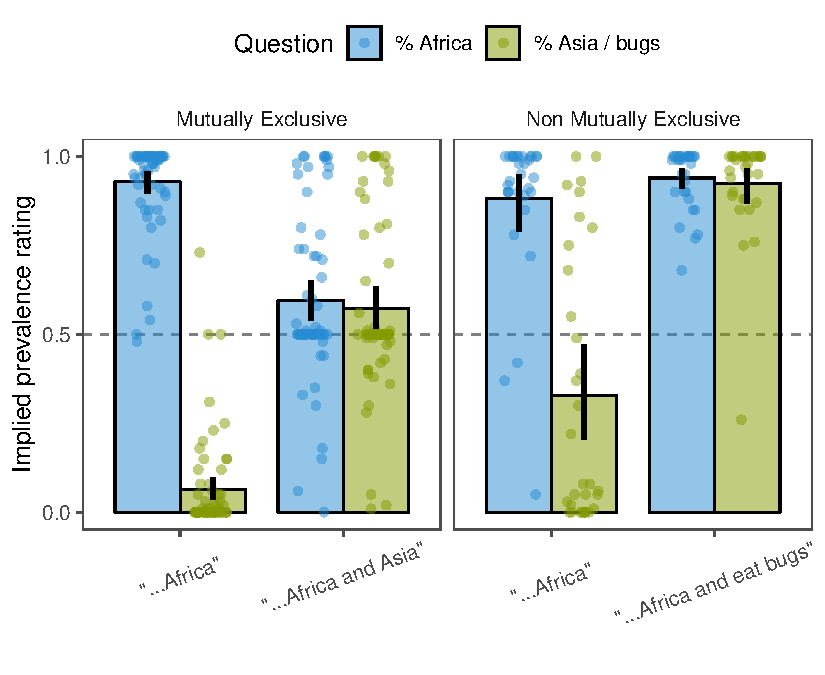
\includegraphics[width=0.5\textwidth]{figs/expt2a_summary.pdf}
    \vspace{-1.25cm}
  \caption{Experiment 1 results.  Participants rate prevalence for mentioned property (\% live in Africa) and either the mutually exclusive property (left facet) or non-mutually exclusive property (right facet), mid sentence (``Africa'') or after the sentence finishes (``Africa and X''). Error-bars denote bootstrapped 95\% confidence intervals.}
  \label{fig:expt2}
          \vspace{-0.5cm}
\end{figure}
 
The results are visually apparent in Fig.~\ref{fig:expt2}.
Reading only ``Elephants live in Africa\ldots'' led listeners to believe, on average, that all elephants lived in Africa and that none lived in Asia, whereas if the sentence finished ``\ldots and Asia'', listeners inferred that roughly half live in Africa and half live in Asia.
This inference is not categorical, however; there are a number of responses to ME conjunctive generics wherein participants  infer that all or almost all have both properties (recall that many of our items are unfamiliar properties).
A different pattern was observed for the NME properties, where hearing about the second property (``eat bugs'') only increased participants' degree of belief in each property applying.
Further, when answering about unmentioned properties, participants rated the prevalence of ME properties close to 0\% whereas NME properties were rated as somewhat prevalent (green bars, ``Africa'').
The results replicate intuitions about how ``Elephants live in Africa'' should be interpreted in a context where the sentence is interrupted. 
The comparison with the non-mutually exclusive condition shows that the results cannot be attributed to the very act of being asked about two properties mentioned in a conjunctive generic sentence.



\subsection{Experiment 2: Strong incrementality}

In Expt.~1, we demonstrated that the mutually exclusive inference effects can be measured using a gating paradigm wherein participants are queried for their beliefs part-way through a sentence. 
Here, we exploit this paradigm to test the strong incremental processing predictions of the model, where syntactic expectations can modulate the interpretations of generic sentences in a fine-grained manner. 
Sample size, participant exclusion criteria, and analyses for this experiment were pre-registered on OSF \url{osf.io/pjt9c}.

\subsubsection{Participants}

We recruited 108 participants through Amazon's Mechanical Turk.
Participants were restricted to those with verified U.S. IP addresses and at least a 95\% work approval rating. 
The study took about 10 minutes and participants were compensated \$1.50.

\subsubsection{Materials and procedure}

The materials and procedure  followed those of Expt.~1 with the following exceptions.
We modified the critical conjunctive generics to primarily involve the conjunction of two noun phrases (e.g., \emph{ascribe to Cabooism and Daithism}) in order to strength the correlation between the NP-conjunction and mutual exclusivity.\footnote{
Of the 13 items in this experiment, 9 of them were NP-coordinated (the others used coordination of prepositional phrases and adjectives).  In both experiments, critical conjunctive generics always involved conjunctions of the same syntactic types (e.g., \emph{ascribe to the Caboo religion and the Daith religion}).
}
The fillers were modified to introduce page breaks immediately before and immediately after conjunctions (``and'') in order to raise participants' expectations that a sentence might be broken at a conjunction.
We used additional examples of the Uninterrupted ME condition of Expt.~1 (``live in Africa and Asia.'') as fillers to raise participants' expectations about ME continuations.
Half of the filler trials had page breaks immediately before the ``and'' and half immediately after.

On critical trials, questions always interrupted the chapter right before the last page.
On the question screen, the page number of the penultimate page remained on the screen to provide an additional cue that the chapter was not complete (Fig.~\ref{fig:design}A).
There were three conditions corresponding to the point in the sentence at which the page break and prevalence questions occurred: ``Elephants live in Africa\_\_ and\_\_ Asia\_\_'' (where \_\_ denotes the page-break).
In the two conditions where participants did not see the full conjunctive property before the question (INT A and A\&), the sentence continued with a non-mutually exclusive property (e.g., \emph{eat bugs}). 

Finally, we changed the question about the second property (\% live in Asia) to ask about ``some other X'', where X was the kind of property that was mentioned in the first conjunct (e.g., \emph{live on some other continent}).
This change was introduced to raise the plausibility that a second, ME property was possible while not  naming one explicitly, which would be pragmatically odd given that the property is unmentioned in the INT A and A\& conditions. 
Participants saw 18 chapters. The story started with a chapter with no questions, then participants saw 4 fillers: 2 quantifiers with interrupting questions and 2 uninterrupted ME fillers, in a random order. Finally, participants saw 2 of each kind of critical trial with 4 uninterrupted ME fillers and 3 quantifier fillers interleaved to avoid back-to-back critical trials. 
 \subsubsection{Results}
\begin{figure}[h]
  \centering
    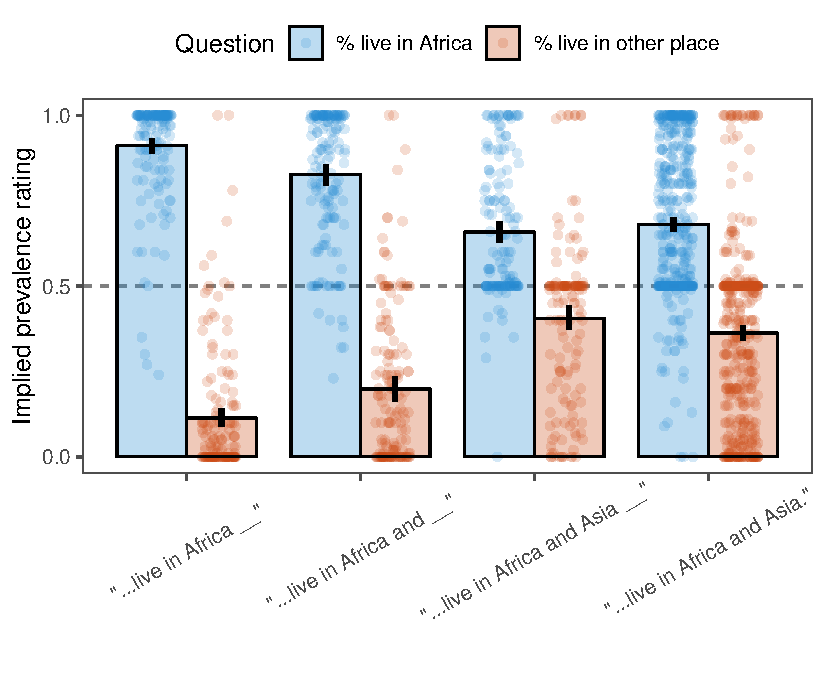
\includegraphics[width=0.5\textwidth]{figs/expt3_summary.pdf}
    \vspace{-1cm}
  \caption{Experiment 2 results. Participants are interrupted at various stages of the sentence (after \emph{Africa}, \emph{and}, or \emph{Asia}) to be asked about the prevalence of \emph{living in Africa} and \emph{living in some other place}, or asked at the end of the sentence (right-most bars). When participants are interrupted before the second conjunct (\emph{Asia}), the sentence continues with a non-mutually exclusive property. Error-bars denote bootstrapped 95\% confidence intervals.}
    \label{fig:expt3}
\end{figure}


28 participants were excluded for failing at least one of the two attention checks.\footnote{
6 failed slider check; 9 failed memory check; 13 failed both.
}
To test our main prediction, we constructed a Bayesian mixed-effects regression model predicting implied prevalence ratings for the first conjunct (e.g., \% Africa) as a function of the point in the sentence in which participants were queried. 
We included by-item and by-participant random intercepts and slopes.\footnote{
model: $\texttt{rating} \sim \texttt{cond} + (1 + \texttt{cond} \mid \texttt{subj}) + (1 + \texttt{cond} \mid \texttt{item})$
}
The regression model was created in Stan (http://mc-stan.org/) accessed with the brms package using default priors \cite{burkner_brms_2017}.


Replicating the findings of Expt.~1, when participants only read that ``Elephants live in Africa'', they tended to infer that almost all lived in Africa. 
When they read that ``Africa and Asia'', they tended to infer that the distribution was close to 50\%-50\%.
Finally, as predicted by a strong version of incremental processing, participants began to anticipate a mutually-exclusive conjunct when only the word ``and'' was mentioned, as evidenced by their implied prevalence ratings being substantially less for the ``..live in Africa and\_\_'' condition than the ``live in Africa'' condition (posterior mean estimate and 95\% credible interval: $\beta = -0.08$ (-0.13, -0.04)).
In addition, these ratings were substantially higher than when the full conjunctive predicate was present ``..live in Africa and Asia'' ($\beta = 0.17$ (0.12, 0.23); Fig.~\ref{fig:expt3}).
Thus, we find that participants' implied prevalence ratings of how many elephants live in Africa monotonically decreased as a function of how many words of the conjunctive predicate they were allowed to see. 
These results suggest that listeners begin to draw pragmatic interpretations of generics before the end of the sentence and even in the absence of additional content words. 

It is notable that in the ``Africa and Asia'' conditions, participants on average infer greater than 50\% prevalence for \emph{Africa} and lower than 50\% for \emph{Asia}, a departure from the results of Expt.~1.
This deviation may be due to participants forgetting what they have read and/or not making the inference that the second conjunct stands in a subset relation to the category in the second question (e.g., that \emph{Asia} is a kind of ``some other continent'').
Explicitly asking about the conjuncts alleviates memory demands by allowing participants to merely recognize, rather than recall, that they have seen this conjunct mentioned. 
Asking about \emph{some other continent} (Expt.~2) requires participants' to recall the second conjunct and could lead to lower prevalence ratings in response to this question.

\section{Discussion}

Generic sentences exhibit extreme sensitivity to context that make it difficult to precisely define what a single generic conveys. 
``Elephants live in Africa and Asia'' means neither that \emph{most elephants live in (both) Africa and Asia} nor that \emph{most elephants live in Africa, and most live in Asia}.
Here, we empirically measured interpretations of generics about conjunctive predicates, building on the observation of \citeA{Nickel2008} of the range of troubling examples for quantificational views of generics.
Notably, the uncertain threshold model of \citeA{Tessler2019:genLang} accounts for such conjunctive generics seamlessly: An underspecified threshold can be updated as more information comes in and is sensitive to prior beliefs regarding compatibility of the conjunct properties.

We extended that model to include syntactic expectations and found evidence for the strongest form of incremental syntactic processing, wherein beliefs are continually updated based on expectations of how a sentence will continue. 
The fact that generic language understanding can be modulated simultaneously by correlations in background knowledge and by syntactic expectations calls for a tighter coupling between models of syntactic processing \cite{Levy2008}, pragmatic language understanding \cite{Goodman2016}, and intuitive theories \cite{tenenbaum2011grow}. 

It remains an open question, however, how specific the effects observed in this paper are to generics rather than to quantification more generally. 
For example, it appears that, in some contexts, one can use \emph{most} to convey similar mutually exclusive conjunctions: ``Elephants are the largest land animal on Earth and are one of the gentlest creatures. Most live in Africa and Asia but are brought to other places for the entertainment of humans.''\footnote{
Example from theodysseyonline.com/want-to-ride-an-elephant
}
Further work is needed to determine the felicity and interpretation of such utterances.

\vspace{0.1cm}
\fbox{\parbox[b][][c]{7.3cm}{\centering Data, code, and links to experiments are available at\ \url{https://github.com/mhtess/elephants}}}


\section{Acknowledgments}

This work was supported by the National Science Foundation Grant \#1456081, Elemental Cognition, and the MIT Sensetime Alliance and Quest for Intelligence. 

\bibliographystyle{apacite}

\setlength{\bibleftmargin}{.125in}
\setlength{\bibindent}{-\bibleftmargin}

\bibliography{elephants}

\appendix
\section{Experiments}
\subsection{Materials}
Critical materials consisted of 13 conjunctive generics. In particular, each chapter presented a novel kind and one predicate. There were two possible continuations, a predicate that was mutually exclusive with the one already presented (ME), and one that was not mutually exclusive with the one already presented (NME). Background information on the kind was presented in order to facilitate the desired inferences about mutual exclusivity. All critical materials are shown in Table \ref{tab:storybookmaterials}.
\begin{table}
\caption{Materials for Experiments 1 and 2, showing the category, the first feature, the corresponding mutually exclusive (ME) feature, and the corresponding non-mutually exclusive (NME) feature.}
\small
\begin{tabular}{p{1.5cm}|p{4.5cm}|p{4.5cm}|p{4.5cm}}
Kind           & Predicate                                      & ME Predicate                        & NME Predicate                 \\ \hline
Ludinos        & ascribe to the Caboo religion                  & ascribe to the Daith religion                       & pray three times a day                           \\
glippets       & live on the northern continent of Caro         & live on the southern continent of Este              & enjoy the sunshine there                         \\
mooks          & have territories at the tops of tall mountains & have territories at the bottom of deep canyons      & watch over the low-lying regions during the day  \\
aliens         & flood their fields to plant fujusi             & burn their fields to plant soroneeks                & spray them with a naturally-occurring fertilizer \\
fengnors       & build their nests in gluers                    & build their nests in droops                         & store tree-bark in them for safe keeping         \\
Krens          & are stup-herders                               & are fishermen                                       & sing songs to the stups to help them relax       \\
lorches        & have long wings                                & have short wings                                    & have sharp claws                                 \\
reesles        & wear wutsats around their heads                & wear krevnors around their heads                    & carry sticks with them                           \\
kweps          & chew on xorfun                                 & chew on tunkel                                      & jump up and down in circles                      \\
ollers         & carry their young in guklags                   & carry their young in trullets                       & are very protective                              \\
basket weavers & are part of the Tinno guild                    & are part of the Farza guild                         & sell their baskets in the Warfi marketplace      \\
batozes        & have six wings                                 & have seven wings                                    & can flap their wings very fast                   \\
kaples         & have striped fur                               & have spotted fur                                    & have long tails                                  \\
landeks        & have four horns                                & have seven horns                                    & have two tails                                   \\
vimble queens  & hibernate in fallen logs                       & hibernate in the abandoned burrows of other animals & give birth twice a year                          \\
isooms         & produce fruit with bumpy skin                  & produce fruit with smooth skin                      & produce fruit with a sour taste                 
\end{tabular}
\label{tab:storybookmaterials}
\end{table}

\subsection{Participants}
Participants were recruited through Amazon Mechanical Turk. In order to ensure data quality, three different checks were performed. 

First, participants were assessed for their understanding of the experimental measure, which was an implied prevalence task. In the implied prevalence task, participants are asked to rate how prevalent a given predicate is in a given kind (e.g. how prevalent is \emph{living in Africa} in the kind of \emph{elephants}). To check for understanding of this measure, participants were asked to rate what percentage of \emph{lions lay eggs}, \emph{cats get cancer}, and \emph{dogs bark}. Participants that did not respond that 

Second, participants were assessed for paying attention. They were presented with 10 statements and asked to classify which of the 10 they had seen or not during the experiment. There were 5 genuine and 5 distractor statements; participants that did not correctly classify 7 of the 10 statements were excluded.

Third, participants were asked for an explanation of what they had done during the experiment.

\subsection{Experimental Design}

\end{document}